% ===========================================================================
%  When Does Test-Time Adaptation Help in Smart Buildings?
%  Standalone manuscript. Every number traces to a script in ../../src and a
%  CSV in ../../results; the "% source:" comment above each table names both.
% ===========================================================================
\documentclass[a4paper,fleqn]{cas-dc}

\usepackage[numbers]{natbib}
\usepackage{amsmath,amssymb}
\usepackage{booktabs}
\usepackage{graphicx}
\usepackage{multirow}
\usepackage{array}

\graphicspath{{./}{figures/}}
\newcommand{\macf}{macro-F\textsubscript{1}}

\makeatletter
\AtBeginDocument{\@ifundefined{printorcid}{}{\renewcommand{\printorcid}{}}}
\makeatother

\begin{document}

\let\WriteBookmarks\relax
\def\floatpagepagefraction{1}
\def\textpagefraction{.001}

\shorttitle{When does test-time adaptation help in smart buildings?}
\shortauthors{M. Kbaier et al.}

\title[mode=title]{When Does Test-Time Adaptation Help in Smart Buildings?
A Protocol-First Evaluation of Three Image-Domain Methods on Two Sensor Tasks}

\author[1]{Mariem Kbaier}
\ead{kbaiermeryem@gmail.com}

\author[1]{Ons Abderrahim}

\author[1]{Manar Amayri}

\author[1]{Nizar Bouguila}
\cormark[1]
\ead{nizar.bouguila@concordia.ca}

\affiliation[1]{organization={Concordia Institute for Information Systems
  Engineering, Concordia University},
  city={Montreal}, state={QC}, country={Canada}}

\cortext[1]{Corresponding author.}

\begin{abstract}
Buildings consume a large share of global energy, and occupancy-aware control depends on
models that keep working after they are installed somewhere new. Test-time adaptation
(TTA) is an attractive answer: a trained model updates itself online from the unlabelled
stream it is already processing, without source data and without annotation from the new
site. The methods that define the area were developed for image corruptions, and whether
their assumptions survive the move to one-dimensional sensor data is an open question.

We evaluate three of them --- DIGA, PETAL and PeTTA --- on two smart-building tasks: human
activity recognition across two instrumented apartments, and occupancy estimation across
two instrumented offices. Because the comparison is only as trustworthy as the protocol
underneath it, we first quantify a measurement problem that is known in the activity
recognition literature but still common in practice. Sliding windows with unit stride make
adjacent samples share nineteen of twenty timesteps, so a random train/validation split
places a near-duplicate of almost every validation sample into training. Under that split
a source model reaches $0.998$ \macf; grouped by recording day it reaches $0.529$. The
window definition accounts for under two points of the difference and the split for
forty-seven. Every result we report uses day-grouped splits.

On that footing the cross-building penalty is asymmetric. Measured against a model trained
on the target building at matched sample size, it is $0.6$ \macf{} points entering one
apartment and $21.3$ entering the other. The three methods track the asymmetry rather than
the task: in the direction with no measurable shift all three lose ground, by $8.6$ to
$20.4$ points, and in the direction with real headroom only DIGA avoids doing so, at
$+2.1$ points with a day-level bootstrap interval of $[-0.8,+4.8]$ that includes zero. The
asymmetry is therefore between losing clearly and not moving detectably. A practitioner cannot know in advance which of the two situations a deployment
is in, since establishing that would require the target labels TTA exists to do without.

The mechanism is shared. All three methods adapt batch-normalisation statistics, and that
channel carries their behaviour: disabling it while leaving everything else intact reduces
PETAL and PeTTA to altering fewer than $25$ predictions of the target stream, and the cost of the
channel rises with the share of target statistics mixed in, from $-5.7$ points at pure
source statistics to $-33.0$ at pure target ones, with the ordering broken only at a single
step in each direction. We also find that the
per-sensor features dominating the conventional design score \emph{below} stratified-random
guessing on the target in both directions, because a given sensor index is a different
physical device in each building.

Occupancy estimation reproduces the pattern on a different task, dataset and sensing
modality, and identifies the same cause independently. Of the nine features shared between the
offices, two correlate with occupancy in one and anti-correlate in the other, one of them
with day-level bootstrap intervals that exclude zero.
Removing them is a diagnostic rather than a deployable configuration, since identifying
which features reverse requires target labels, but it isolates the cause: it moves
cross-office transfer from MCC $-0.38$ to $+0.43$ and cuts the measured penalty in one
direction from $47.2$ points to $7.6$. Against the checkpoint whose predictions those
features undermine, PETAL and PeTTA gain over $50$ MCC points. Under the label-free
protocol both lose against the sound checkpoint in the other direction; restricting the
analysis to the seven diagnostic features leaves no broken checkpoint and reduces every
method's effect to at most $12$ points. We conclude that in this domain the effectiveness of test-time adaptation is
governed by the quality of the checkpoint being adapted and by the reliability of the
measurement, more than by the merits of the adaptation method.
\end{abstract}

\begin{keywords}
Test-time adaptation \sep Human activity recognition \sep Occupancy estimation
\sep Smart buildings \sep Evaluation protocol
\end{keywords}

\maketitle

% ============================================================================
\section{Introduction}
\label{sec:intro}

Buildings account for a large share of global energy demand, and occupancy-aware control of
heating, ventilation and lighting is among the more direct levers available for reducing
it \cite{manfren2021,amangeldy2025}. Human activity recognition (HAR) and occupancy
estimation (OE) supply the signal such control needs \cite{dridi2022,amayri2019}. Both are
learned from sensor traces, and both face the same obstacle when a model trained in one
building is installed in another: room layouts differ, sensors sit in different places, and
occupants keep different routines \cite{hong2017,shahbazian2023}. A model that works where
it was trained often does not work in the next building.

Test-time adaptation addresses this without requiring labels from the new site. A frozen
source model updates itself online from the unlabelled stream it is already processing,
with no access to source data and no target annotation \cite{liang2024}. For buildings,
where sensors are always on and manual annotation is impractical, the fit is obvious. The
method family has matured quickly on images: DIGA \cite{diga} adapts normalisation
statistics and class prototypes without gradients, PETAL \cite{petal} treats lifelong
adaptation as probabilistic inference, and PeTTA \cite{petta} stabilises adaptation when
environments recur. Whether their assumptions survive the move to one-dimensional sensor
data is an open question, and the one we set out to answer.

Answering it requires first establishing that the quantity these methods are asked to
reduce is measured soundly, and we begin there. Features in this literature are computed
over sliding windows with unit stride, so consecutive samples share nineteen of their
twenty timesteps, and a random train/validation split places a $95\%$-identical copy of
nearly every validation sample into training. That overlapping windows bias cross-validation
in activity recognition is established \cite{hammerla2015}; what we add is the magnitude on
this pipeline and the separation of the split from the window definition. We then evaluate
the three methods on two tasks under the corrected protocol.

Our contributions are as follows.

\begin{itemize}
\item \textbf{A trustworthy evaluation protocol for this data type.} We isolate the
  measurement problem by varying the window definition and the validation split
  independently. Causality and segmentation move source \macf{} by under two points; the
  split moves it by forty-seven (Section~\ref{sec:protocol}). Everything thereafter uses
  day-grouped splits, and the cross-building penalty is measured against a model trained on
  the target building at matched sample size rather than against source validation.

\item \textbf{A rigorous evaluation of DIGA, PETAL and PeTTA across two tasks.} Both
  transfer directions, both tasks, published hyperparameters, chance baselines and paired
  bootstrap intervals throughout (Sections~\ref{sec:har} and~\ref{sec:occ}). The three
  methods track the measured penalty rather than the task: they lose ground clearly where
  there is none, and where there is headroom the best of them is not distinguishable from
  doing nothing.

\item \textbf{A cross-task-confirmed account of why source models fail to transfer.}
  On activity recognition, features tied to a sensor index score below stratified-random
  guessing in both directions. On occupancy, two features correlate with occupancy in one
  office and anti-correlate in the other, one of them with day-level intervals that exclude
  zero, and removing both --- a diagnostic, since identifying them requires target labels
  --- changes the sign of the transfer result.
  The same failure --- a feature whose meaning is specific to one installation --- is found
  independently on two tasks, two datasets and two sensing modalities.
\end{itemize}

Section~\ref{sec:related} reviews domain adaptation and TTA for sensor data.
Section~\ref{sec:data} describes the data and the three methods.
Section~\ref{sec:protocol} establishes the protocol. Sections~\ref{sec:har}
and~\ref{sec:occ} report the two evaluations. Sections~\ref{sec:discussion}
and~\ref{sec:conclusion} discuss and conclude.

% ============================================================================
\section{Related work}
\label{sec:related}

\subsection{Domain adaptation in smart buildings}

Transferring occupancy and activity models between rooms has been studied extensively by
Dridi and colleagues, through fine-tuning and layer freezing \cite{dridi2022}, unsupervised
adaptation with and without source access \cite{dridi_sfda}, and clustering-based
alignment \cite{dridi_cluster}. Abderrahim et al.\ extend the setting to open and universal
label spaces \cite{abderrahim2025,abderrahim2026}. These works establish that cross-room
transfer is a real and recurring problem in this domain. They generally assume source data
remains available, or that adaptation may run offline over the full target set, neither of
which holds for a streaming deployment.

\subsection{Test-time adaptation and its assumptions}

Test-time adaptation drops both assumptions: the source model is frozen, source data is
unavailable, and adaptation proceeds online over the target stream
\cite{liang2024,tent,cotta,shot}. The price is a set of implicit assumptions about what the
shift looks like. Most of the family adapts normalisation statistics, which presumes the
shift is largely a change in the first two moments of the features, and most presumes a
test stream long enough for a slowly-updated teacher to move. Both presumptions are
comfortable on image corruption benchmarks, where a corruption shifts an entire feature
distribution coherently and a single corruption supplies tens of thousands of images.
Neither is obviously safe when the shift is a change of building.

\subsection{TTA for one-dimensional data}

Work applying TTA to sensor streams is comparatively thin. Wang et al.\ report an
optimisation-free method for cross-person activity recognition \cite{wang2023}. What is
largely missing is an account of how evaluation protocol and feature design interact with
measured adaptation gains, which is the gap this paper addresses. The closest prior
evidence on the protocol side is Hammerla and Pl\"otz \cite{hammerla2015}, who show that
pairwise similarity between overlapping windows biases cross-validation in activity
recognition. That finding is a decade old and the practice it warns against remains
common; Section~\ref{sec:protocol} quantifies what it costs on the present pipeline.

% ============================================================================
\section{Data, model and methods}
\label{sec:data}

\subsection{Activity recognition}

The dataset of Tapia et al.~\cite{tapia2004} provides two single-occupant apartments,
denoted $\text{S}_1$ and $\text{S}_2$, instrumented with binary proximity sensors placed on
household objects and furniture and sampled at $30$~s. We use the five activities common to
both: \texttt{toileting}, \texttt{meal\_prep}, \texttt{watching\_tv}, \texttt{music} and
\texttt{cleaning}. After windowing there are $5031$ samples from $\text{S}_1$ over $16$
recording days and $3412$ from $\text{S}_2$, with $53$ sensor channels shared between the
two apartments. Class sizes are uneven; \texttt{cleaning} has $442$ windows in
$\text{S}_1$ and $113$ in $\text{S}_2$.

\subsection{Occupancy estimation}

The occupancy data comes from two offices at the Grenoble Institute of Technology,
instrumented with a carbon dioxide sensor, a motion counter, an acoustic
level (\texttt{rms}), door and window contacts, and several sub-metered power channels,
sampled at $10$~minutes. The source office contributes $1210$ samples over $10$ recording
days and the target office $1041$ over $8$. Labels are occupant counts, which we binarise
to occupied against unoccupied; the positive rate is $33.5\%$ and $28.0\%$ respectively.
Nine feature columns are common to both offices. This data is not ours to redistribute.

\subsection{Model}

All experiments use the same classifier: a three-layer perceptron with batch normalisation,
ReLU and dropout at each layer, widths $256$--$128$--$64$, and a linear output. The
architecture is held fixed throughout so that differences between conditions are not
confounded by capacity. Source checkpoints are selected by held-out \macf{} under the
protocol of Section~\ref{sec:protocol}.

\subsection{Adaptation methods}

We evaluate three methods, each implemented from the equations and hyperparameters of its
source paper and run at the configuration its released implementation uses.

\textbf{DIGA} \cite{diga} adapts without gradients. Its distribution adaptation module
mixes frozen source batch-norm statistics with those of the current test batch under a
weight $\lambda_{BN}$, and its semantic adaptation module maintains class prototypes from
confident predictions and fuses a prototype-based posterior with the classifier's.

\textbf{PETAL} \cite{petal} treats lifelong adaptation as probabilistic inference. A
student is updated against pseudo-labels from an exponential-moving-average teacher, with a
term pulling the weights toward a SWAG posterior fitted on the source, and a
Fisher-information criterion restoring parameters whose importance falls below a threshold.

\textbf{PeTTA} \cite{petta} targets recurring test environments. It maintains a
category-balanced memory bank and senses divergence from the source feature distribution,
using that signal to modulate both the teacher update rate and the strength of an anchor
loss.

Two further methods appear throughout as \emph{reference baselines} rather than as methods
under evaluation. \textbf{AdaBN} replaces the source normalisation statistics with those of
the test batch and does nothing else; \textbf{TENT} \cite{tent} adds entropy minimisation
over the normalisation parameters. They are included because the three evaluated methods
all contain a normalisation-adaptation component, and isolating what that component
contributes requires a method that contains nothing else.

\subsection{Metrics}

Classes are unbalanced in both tasks, so we report macro-F\textsubscript{1} and Matthews
correlation coefficient rather than accuracy alone, with accuracy and balanced accuracy
beside them for the binary task. Two chance baselines accompany every activity result:
stratified-random sampling from the target class distribution, and the majority class.
Intervals on differences are paired bootstraps over the target stream, resampled at the
level of the recording day rather than the individual window or record. Windows computed
over overlapping spans are not independent draws (Section~\ref{sec:protocol}), and
consecutive occupancy records are strongly autocorrelated, so resampling them individually
treats dependent observations as independent evidence and narrows every interval it
produces.

% source: src/exp36_diga_ci.py -> results/exp36_diga_ci.csv, both resampling units

% ============================================================================
\section{Establishing a trustworthy protocol}
\label{sec:protocol}

Features in this literature are computed over a sliding window advanced one sample at a
time. At the window length of $W=20$ used here, consecutive feature vectors are built from
overlapping spans sharing nineteen of twenty timesteps, so neighbouring samples are close
to duplicates of one another. A validation split drawn at random over such a sequence
therefore places a near-copy of almost every validation sample into the training set, and
the resulting score measures memorisation rather than generalisation. Hammerla and
Pl\"otz \cite{hammerla2015} identified this effect in activity recognition a decade ago.
Our purpose here is to quantify what it costs on the present pipeline and to separate it
from a second choice it is easily confused with, namely how the window itself is defined.

Two choices are varied independently. The first is causality: whether the window centred on
a labelled sample extends symmetrically in both directions, which lets a feature read five
minutes into the future and contradicts the online premise of test-time adaptation, or
extends backwards only, which is what a deployed system can compute. The second is the
validation split: random over samples, blocked into contiguous runs, or grouped by
recording day so that no day contributes to both sides.

% source: src/exp4_windowing.py -> results/exp4_windowing.csv, 5 seeds
\begin{table}[t]
\centering
\caption{Source-domain \macf{} on $\text{S}_1$ under three validation splits, with the
window definition held fixed. Target performance is unchanged across all three, so the
difference is entirely in what the source figure measures.}
\label{tab:protocol}
\small
\begin{tabular}{@{}lcc@{}}
\toprule
Validation split & Source \macf & Target \macf \\
\midrule
Random over samples & $0.9984\pm0.001$ & $0.1626$ \\
Blocked into runs   & $0.4431\pm0.018$ & $0.1626$ \\
Grouped by recording day & $\mathbf{0.5287}\pm0.007$ & $0.1626$ \\
\bottomrule
\end{tabular}
\end{table}

% source: src/make_figures_final.py, values transcribed from Table~\ref{tab:protocol}
\begin{figure*}[t]
\centering
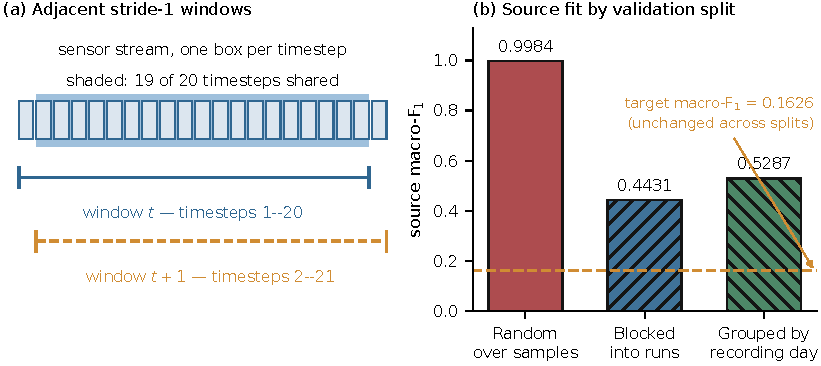
\includegraphics[width=0.96\textwidth]{fig_leakage.pdf}
\caption{Overlapping-window leakage. Left: adjacent stride-$1$ windows share $19$ of
$20$ timesteps. Right: source \macf{} under three validation splits; the window
definition accounts for under two points of the difference, the split for forty-seven.}
\label{fig:leakage}
\end{figure*}

Table~\ref{tab:protocol} and Figure~\ref{fig:leakage} separate the two. Changing the window definition --- causal
against centred, and how segments are delimited --- moves the source figure by under two
points. Changing the split moves it by forty-seven, from $0.9984$ to $0.5287$. The inflation
is a property of the split, not of the window, and a pipeline that fixes the window while
leaving the split random retains essentially all of it.

The practical consequence is that a cross-building drop computed as source validation minus
target performance is not a measurement of two buildings. Under the random split that
difference is $84$ points on this data, almost all of which is the source figure being
wrong. We therefore adopt grouped-by-day splits for every result that follows, and we make
windows causal, which is required anyway if the features are to be computable online. The
second change is not a trade: causal windows improve target \macf{} from $0.1626$ to
$0.2356$, because a centred window straddling an activity boundary mixes two activities.

A further consequence shapes Section~\ref{sec:har}. If source validation cannot be trusted
as a reference point, then the cross-building penalty should not be computed against it.
We instead hold the evaluation set fixed and vary only where the training labels came from,
comparing a model trained on the target building's own days with one trained on the source
building, at matched training-set size. That quantity is the price of not having labels in
the new building, which is what test-time adaptation is asked to recover.

% ============================================================================
\section{Activity recognition}
\label{sec:har}

\subsection{Sensor identity does not transfer}
\label{sec:har-feat}

The conventional feature vector for this data devotes most of its dimensions to per-sensor
statistics: the mean and standard deviation of each sensor channel over the window. Such a
feature encodes which device fired. Sensor index $100$ is a different physical device in
each apartment, so a rule learned about it is not merely uninformative in the other
building but wrong.

% source: src/exp11_reverse.py -> results/exp11_reverse.csv, 3 seeds x 5 folds
\begin{table}[t]
\centering
\caption{Target \macf{} by feature set, both transfer directions, causal features and
day-grouped source selection. Stratified-random guessing scores $0.200$ in both
directions; figures below it are in bold.}
\label{tab:harfeat}
\small
\begin{tabular}{@{}llcc@{}}
\toprule
Feature set & $d$ & $\text{S}_1\!\to\!\text{S}_2$ & $\text{S}_2\!\to\!\text{S}_1$ \\
\midrule
Layout-invariant & $13$ & $\mathbf{0.4466}$ & $\mathbf{0.3068}$ \\
No per-sensor & $29$ & $0.3630$ & $0.2271$ \\
Conventional (all) & $135$ & $0.2118$ & $\mathbf{0.1583}$ \\
Per-sensor only & $106$ & $\mathbf{0.1350}$ & $\mathbf{0.1702}$ \\
\midrule
Stratified random & --- & $0.1997$ & $0.2003$ \\
\bottomrule
\end{tabular}
\end{table}

Table~\ref{tab:harfeat} measures the consequence. Per-sensor features alone score $0.1350$
and $0.1702$ against a stratified-random baseline of approximately $0.200$: below chance in
both directions. They are not weakly informative; a model built on them is systematically
wrong in the other apartment. The conventional $135$-dimensional vector, which is dominated
by them, falls below chance in one direction as well.

Replacing them with thirteen window-level summary statistics that describe how much
activity is occurring and when, without naming any sensor, raises target \macf{} to $0.4466$
and $0.3068$. That is the checkpoint used for everything that follows.

How that set was arrived at should be stated, because it bears on how the figure may be
read. The \emph{motivation} is prior to any measurement: a feature naming a sensor index
cannot transfer, since the index identifies a different device in each apartment, and that
follows from how the data was collected rather than from any result. The \emph{specific
choice} among the candidate sets in Table~\ref{tab:harfeat} was not blind, however. We
evaluated several groupings and retained the one with the best target \macf, so target
labels informed the selection even though no individual model was trained on them. The
$0.4466$ and $0.3068$ figures are therefore the best of several candidates rather than a
single pre-registered choice, and should be read as such. Two things limit how much this
matters here. The ordering is not close --- the retained set leads the next candidate by
$5.1$ points entering $\text{S}_2$ --- and the result that carries the argument is the
per-sensor set falling \emph{below} a chance baseline, which is a comparison against
stratified-random guessing rather than against the other candidates and so does not depend
on the selection at all. The result parallels
the general principle that a feature tied to a specific installation cannot transfer, and
Section~\ref{sec:occ-feat} finds the same principle at work on a different task and
modality.

\subsection{The cross-building penalty is asymmetric}
\label{sec:har-gap}

% source: src/exp21_domain_gap.py -> results/exp21_matched.csv, 3 seeds x 5 folds
\begin{table}[t]
\centering
\caption{Cross-building penalty on a fixed evaluation set at matched training-set size.
\emph{Own days} trains on the apartment being evaluated; \emph{other building} trains on
the other one. The difference is what a deployment pays for having no labels in the new
building.}
\label{tab:hargap}
\small
\begin{tabular}{@{}lccc@{}}
\toprule
Evaluated on & Own days & Other building & Penalty \\
\midrule
$\text{S}_2$ held-out days & $0.3497$ & $0.3434$ & $\mathbf{0.6}$ pts \\
$\text{S}_1$ held-out days & $0.4897$ & $0.2767$ & $21.3$ pts \\
\bottomrule
\end{tabular}
\end{table}

% source: src/make_figures_final.py, values transcribed from Table~\ref{tab:hargap}
\begin{figure}[t]
\centering
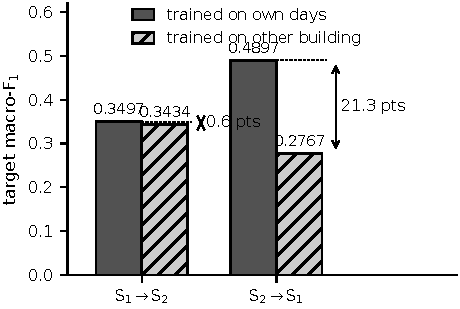
\includegraphics[width=\columnwidth]{fig_penalty.pdf}
\caption{The cross-building penalty is asymmetric: negligible entering $\text{S}_2$,
substantial entering $\text{S}_1$.}
\label{fig:penalty}
\end{figure}

Table~\ref{tab:hargap} and Figure~\ref{fig:penalty} report the penalty measured as described in
Section~\ref{sec:protocol}. It is not one number. Entering $\text{S}_2$ it is $0.6$ points,
which against a between-fold standard deviation of $0.15$ is not distinguishable from
zero: a model that has never seen $\text{S}_2$ performs on $\text{S}_2$ as well as a model
trained on $\text{S}_2$'s own days. Entering $\text{S}_1$ the same comparison costs $21.3$
points.

This asymmetry organises the rest of this section, and it is worth being explicit about why
both directions are reported rather than the more favourable one. In the direction with no
measurable shift there is nothing for an adaptation method to recover, so any movement it
produces can only be downward. A reader might reasonably ask why a practitioner would not
simply deploy in the favourable direction. The answer is that the favourable direction is
not identifiable in advance. Establishing which of the two situations a given deployment is
in requires measuring the penalty, and measuring the penalty requires labels in the target
building --- which is precisely the thing test-time adaptation exists to avoid needing. A
practitioner installing a model in a new building faces an unknown draw from this
distribution of outcomes. Evaluating only the direction that happens to have headroom would
therefore report a best case as though it were the expected one. Reporting both is not a
limitation of the study; it is the result.

\subsection{Method results and a shared mechanism}
\label{sec:har-methods}

% source: src/exp23_bn_channel.py -> results/exp23_bn_channel.csv, 3 seeds
\begin{table*}[t]
\centering
\caption{Target \macf{} for the three methods and the two reference baselines, both
directions, published settings. $\Delta$ is against source-only in the same direction;
\emph{changed} counts altered predictions, out of $3412$ target windows for
$\text{S}_1\!\to\!\text{S}_2$ and $5031$ for $\text{S}_2\!\to\!\text{S}_1$, since the
target stream is the whole of the other apartment in each case. The lower block disables
the normalisation-adaptation channel while leaving everything else unchanged.}
\label{tab:harmethods}
\small
\begin{tabular}{lcccccc}
\toprule
 & \multicolumn{3}{c}{$\text{S}_1\!\to\!\text{S}_2$ (penalty $0.6$)} & \multicolumn{3}{c}{$\text{S}_2\!\to\!\text{S}_1$ (penalty $21.3$)} \\
\cmidrule(lr){2-4}\cmidrule(lr){5-7}
Method & \macf & $\Delta$ & changed & \macf & $\Delta$ & changed \\
\midrule
Source-only & $0.4944$ & --- & $0$ & $0.3226$ & --- & $0$ \\
\addlinespace[2pt]
DIGA  & $0.4088$ & $-8.6$  & $1279$ & $0.3438$ & $+2.1$ & $1031$ \\
PETAL & $0.3113$ & $-18.3$ & $1739$ & $0.2028$ & $-12.0$ & $3105$ \\
PeTTA & $0.2908$ & $-20.4$ & $1845$ & $0.2158$ & $-10.7$ & $3164$ \\
\addlinespace[2pt]
AdaBN \emph{(baseline)} & $0.3139$ & $-18.0$ & $1784$ & $0.2137$ & $-10.9$ & $3143$ \\
TENT \emph{(baseline)}  & $0.3141$ & $-18.0$ & $1782$ & $0.2133$ & $-10.9$ & $3142$ \\
\midrule
\multicolumn{7}{l}{\emph{normalisation channel disabled, everything else identical}} \\
\addlinespace[2pt]
PETAL & $0.4947$ & $+0.0$ & $11$ & $0.3224$ & $-0.0$ & $24$ \\
PeTTA & $0.4947$ & $+0.0$ & $5$  & $0.3225$ & $-0.0$ & $13$ \\
\bottomrule
\end{tabular}
\end{table*}

Three source checkpoints appear in this section, and they are deliberately different
because they answer different questions. Table~\ref{tab:hargap} compares a model trained on
the target building's own days against one trained on the source building, with both
training sets subsampled to the same size and both scored on the same held-out days.
Equalising the sample count is what isolates the cost of having no labels in the new
building from the separate effect of having less data, and it is why that table's
``other building'' figure ($0.3434$ entering $\text{S}_2$, from $2184$ training samples) is
lower than the checkpoint a deployment would actually use. Table~\ref{tab:harmethods}
reports that deployable checkpoint instead: trained on the full source split and scored over
the entire target stream in a single pass, since a streaming adapter carries state and
cannot be averaged across folds without resetting it. Table~\ref{tab:harfeat}'s figure is a
third quantity again, the full source split averaged over five folds with causal smoothing
applied, which is the best available estimate of deployable accuracy for a feature set. The
three values entering $\text{S}_2$ --- $0.3434$, $0.4944$ and $0.4466$ --- differ by
training-set size, fold averaging and smoothing, not by any disagreement about what is being
scored. Only Table~\ref{tab:harmethods}'s figure is the starting point the adaptation
methods are given.

Table~\ref{tab:harmethods} gives the main activity result. In the direction where the
penalty is $0.6$ points, all three methods lose ground, by $8.6$ to $20.4$ \macf{} points.
In the direction where it is $21.3$, DIGA is the only method that does not clearly lose
ground, at $+2.1$ points, though a paired bootstrap resampled by recording day puts that
difference at $[-0.8,+4.8]$ and so does not separate it from zero. The losses are of a
different character: DIGA's $-8.6$ in the first column has an interval of $[-13.7,-2.8]$
under the same procedure, excluding zero. The methods track the measured penalty rather
than the task, and the asymmetry is between losing clearly and not moving detectably
rather than between losing and gaining.

The resampling unit matters for that statement and is worth making explicit. Resampling
individual windows rather than days would put DIGA's difference at $[+1.4,+2.7]$ and make
it appear significant. That is the effect of Section~\ref{sec:protocol} reappearing in a
different guise: windows sharing nineteen of twenty timesteps are not independent draws,
and treating them as such narrows an interval for the same reason it inflated a
source-validation score. Every interval in this paper resamples the recording day.

The lower block identifies why. All three methods adapt batch-normalisation statistics, and
in each released implementation that is the primary mechanism rather than an incidental
detail. Disabling that channel and leaving every other component untouched --- the
gradient updates, the posterior regularisation, the divergence gating, the memory bank ---
reduces PETAL to altering $11$ predictions of $3412$ entering $\text{S}_2$ and $24$ of
$5031$ entering $\text{S}_1$, and PeTTA to $5$ and $13$. Whatever those components contribute, it is not visible
at this scale. With the channel active, PETAL falls within $0.3$ points of plain AdaBN and
PeTTA within $2.3$, having changed much the same predictions.

% source: src/exp23_bn_channel.py, DIGA with lam_bn swept
\begin{table}[t]
\centering
\caption{DIGA as $\lambda_{BN}$ moves from source statistics ($1.0$) to target statistics
($0.0$), $\Delta$\macf{} against source-only. At $\lambda_{BN}=1.0$ the statistics are
untouched, so that row isolates the prototype classifier from the normalisation; its
day-level bootstrap intervals are $[-8.9,-2.1]$ and $[+1.4,+7.4]$.}
\label{tab:bndial}
\small
\begin{tabular}{@{}lcc@{}}
\toprule
$\lambda_{BN}$ & $\text{S}_1\!\to\!\text{S}_2$ & $\text{S}_2\!\to\!\text{S}_1$ \\
\midrule
$1.0$ (source) & $-5.7$ & $\mathbf{+4.4}$ \\
$0.9$ & $-6.5$ & $+2.4$ \\
$0.8$ (published) & $-8.6$ & $+2.1$ \\
$0.6$ & $-23.3$ & $-12.9$ \\
$0.4$ & $-30.3$ & $-19.9$ \\
$0.2$ & $-25.9$ & $-22.8$ \\
$0.0$ (target) & $-33.0$ & $-20.5$ \\
\bottomrule
\end{tabular}
\end{table}

% source: src/make_figures_final.py, values transcribed from Table~\ref{tab:bndial}
\begin{figure}[t]
\centering
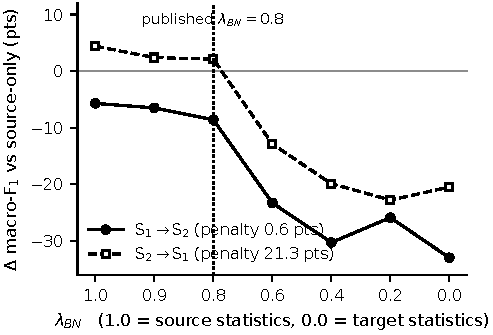
\includegraphics[width=\columnwidth]{fig_bndial.pdf}
\caption{Cost of the shared normalisation-adaptation mechanism. Moving from source
statistics ($\lambda_{BN}=1.0$) to target statistics ($\lambda_{BN}=0.0$) degrades
performance in both directions. The trend is not strictly monotone: the curve recovers
by $4.4$ points between $\lambda_{BN}=0.4$ and $0.2$ in one direction and by $2.3$ points
between $0.2$ and $0.0$ in the other.}
\label{fig:bndial}
\end{figure}

The channel is a continuum rather than a switch, and DIGA's $\lambda_{BN}$ exposes it
directly. Table~\ref{tab:bndial} and Figure~\ref{fig:bndial} sweep it. The cost rises
with the share of target statistics mixed in, in both directions, and steeply: moving from
the published $0.8$ to $0.6$ costs about fifteen points either way. The trend is not
strictly monotone. Entering $\text{S}_2$ the curve recovers by $4.4$ points between
$\lambda_{BN}=0.4$ and $0.2$ before falling again, and entering $\text{S}_1$ it recovers by
$2.3$ points between $0.2$ and $0.0$. Both reversals occur where the source statistics have
been almost entirely displaced and the model is performing near or below chance, so we read
them as noise in a degenerate regime rather than as structure; the overall direction of the
relationship is unambiguous. The top row is also informative. At
$\lambda_{BN}=1.0$ the statistics are exactly the source model's, yet $1026$ predictions
change, because DIGA's prototype classifier is still active. That row is the only
configuration in this study where an adaptation component helps by more than a point
without target labels, and it helps in the direction with headroom and hurts in the
direction without. What stops DIGA from losing ground in that direction is therefore its prototype
classifier, worth $4.4$ points at this setting with a day-level bootstrap interval of
$[+1.4,+7.4]$ that excludes zero, partly spent back by a normalisation step costing $2.3$.
The component gain is therefore established where the method's net effect is not: the
prototype classifier separates from zero, the full method at its published
$\lambda_{BN}=0.8$ does not, and the difference between them is the normalisation step. In
the other direction the same configuration loses $5.7$ points, interval
$[-8.9,-2.1]$, so the component helps only where there is headroom.

One objection deserves pre-empting: that the methods were simply not tuned. As a
post-hoc robustness check only --- and explicitly not part of the label-free protocol used
for every other result in this paper --- we additionally swept each method's own published
hyperparameter grid in both directions, $64$ configurations for DIGA, $24$ for PETAL and
$16$ for PeTTA. Identifying a best configuration requires scoring each one against target
\macf, so this analysis uses target labels that no other result here touches; it bounds
what tuning could achieve rather than reporting something a deployment could obtain.

The conclusion does not move. In the direction without headroom, $53$ of DIGA's $64$
settings lose ground and the best available --- selected with target labels, and therefore
an upper bound --- gains $1.1$ points. No setting anywhere in PETAL's or PeTTA's published
space alters more than $38$ predictions of the target stream, so their behaviour is a property of the
update rules rather than of the configuration. Every figure reported outside this paragraph
uses each method's published settings with no target information of any kind.

% ============================================================================
\section{Occupancy estimation}
\label{sec:occ}

This section asks whether the activity result is a property of that dataset or of the
problem. The task changes from five-class activity recognition to binary occupancy, the
sensing changes from binary proximity switches to carbon dioxide, acoustics, motion and
sub-metered power, the environments change from apartments to offices, and the data comes
from a different institution. If the pattern of Section~\ref{sec:har} is about
cross-building transfer rather than about one dataset, it should reappear.

\subsection{The penalty, and a feature that means two different things}
\label{sec:occ-feat}

% source: src/exp32_occ_feature_identity.py -> results/exp32_occ_feature_identity.csv
\begin{table}[t]
\centering
\caption{Correlation with occupancy per office, with $95\%$ bootstrap intervals over
$2000$ resamples drawn at the level of the \emph{recording day}, since consecutive
occupancy records are strongly autocorrelated. \texttt{rms} is $[+0.561,+0.857]$ against
$[-0.509,+0.029]$ and \texttt{derivative\_co2} is $[+0.038,+0.188]$ against
$[-0.375,-0.066]$; only the latter has intervals of opposite sign that exclude zero, and
is shown in bold on that basis. \texttt{rms}'s source figure is bold as the largest single
correlation in that column.}
\label{tab:occfeat}
\footnotesize
\setlength{\tabcolsep}{3pt}
\begin{tabular}{@{}lcc@{}}
\toprule
Feature & Source office & Target office \\
\midrule
\texttt{sum\_power} & $+0.502$ & $+0.780$ \\
\texttt{co2}        & $+0.378$ & $+0.671$ \\
\texttt{power1}     & $+0.352$ & $+0.462$ \\
\texttt{motion}     & $+0.348$ & $+0.544$ \\
\texttt{power2}     & $+0.263$ & $+0.423$ \\
\texttt{door}       & $+0.255$ & $+0.307$ \\
\texttt{power3}     & $+0.130$ & $+0.721$ \\
\midrule
\texttt{rms}             & $\mathbf{+0.626}$ & $-0.202$ \\
\texttt{derivative\_co2} & $\mathbf{+0.116}$ & $\mathbf{-0.207}$ \\
\bottomrule
\end{tabular}
\end{table}

Table~\ref{tab:occfeat} reports how each shared feature relates to occupancy in each
office. Seven behave consistently. Two do not. The acoustic level \texttt{rms} is the
strongest single predictor the source office has, at $+0.626$, and in the target office it
points the other way at $-0.202$. The rate of change of carbon dioxide does the same more
weakly, at $+0.116$ against $-0.207$.

The evidence for the two is not equally strong, and the resampling unit is what separates
them. Intervals here are drawn at the level of the recording day rather than the
individual record, for the reason Section~\ref{sec:protocol} gives: consecutive readings
from an office are strongly autocorrelated --- an unoccupied room produces near-identical
measurements for hours --- so resampling records treats dependent observations as
independent evidence. At that unit \texttt{derivative\_co2} separates, with
$[+0.038,+0.188]$ against $[-0.375,-0.066]$, while \texttt{rms} does not: its target
interval is $[-0.509,+0.029]$ and includes zero. With eight and ten recording days
respectively, these offices supply few independent units, and the point estimates are far
apart while the intervals around them are wide. We therefore report the reversal as
established for \texttt{derivative\_co2} and as indicated but not established for
\texttt{rms}, and note that resampling individual records would have placed
\texttt{rms}'s target interval at $[-0.314,-0.114]$ and made it appear decisive.

The seven-feature set that appears below is defined by removing these two columns, and
how that set is identified matters for how its rows may be read. Deciding that either feature
reverses requires its correlation with occupancy in \emph{both} offices, and the target
office's correlation is computed from target labels. Every ``$7$ transferable''
row in this section is therefore a diagnostic: it bounds what a correctly-specified feature
set could achieve and isolates the cause of the deficit, but it is not a configuration a
deployment could have selected, because selecting it requires the labels the Tier-1 protocol
forbids. The ``$9$ shared'' rows are the label-free result. We keep both because the
contrast between them is what identifies the mechanism, and we mark the distinction wherever
the seven-feature figures appear.

It is worth being precise about what kind of defect this is, because the obvious
description is wrong. These are not noisy features to be pruned. Removing both drops the
source office's own-days MCC from $0.7643$ to $0.3624$, so nearly half of what that office
knows about its own occupancy is carried by a feature that means the opposite thing next
door. The feature is genuinely predictive at home and genuinely misleading away. That
combination is exactly what makes it invisible to any evaluation conducted in a single
building, and it is why the defect survives into a cross-building result rather than being
caught upstream.

This is the same failure as Section~\ref{sec:har-feat}, reached independently. There the
quantity that did not transfer was a sensor index; here it is a sensor placement. In both
cases a feature encodes something specific to one installation, and in both cases the
consequence is not a weaker model elsewhere but a wrong one.

% source: src/exp33_occ_penalty_raw.py -> results/exp33_occ_penalty_raw.csv, 5 seeds
\begin{table}[t]
\centering
\caption{Cross-office penalty in MCC, day-grouped folds and matched training-set size,
measured exactly as in Table~\ref{tab:hargap}. The $7$-transferable rows are a DIAGNOSTIC:
identifying which two features to drop uses target labels, so they bound what a corrected
feature set could achieve rather than reporting a label-free result.}
\label{tab:occgap}
\footnotesize
\setlength{\tabcolsep}{4pt}
\begin{tabular}{@{}llccc@{}}
\toprule
Features & Evaluated on & Own days & Other office & Penalty \\
\midrule
All $9$ & target & $0.7867$ & $0.2138$ & $57.3$ \\
All $9$ & source & $0.7643$ & $0.2924$ & $47.2$ \\
\addlinespace[2pt]
$7$ transf. & target & $0.8225$ & $0.3777$ & $44.5$ \\
$7$ transf. & source & $0.3624$ & $0.2866$ & $\mathbf{7.6}$ \\
\bottomrule
\end{tabular}
\end{table}

Table~\ref{tab:occgap} applies the measurement of Section~\ref{sec:protocol} to this task;
the raw sensor records carry timestamps, giving ten recording days in the source office and
eight in the target. The penalty is again asymmetric, and dropping the two columns of
Table~\ref{tab:occfeat} cuts it into the source office from $47.2$ points to $7.6$. Most of what presented
as a cross-office domain gap in that direction was two features meaning opposite things in
the two rooms. Into the target office a penalty of $44.5$ points survives the same surgery,
so unlike the apartment pair these two environments do contain a real shift in one
direction.

\subsection{The methods reproduce the pattern}
\label{sec:occ-methods}

% source: src/exp35_occ_tta_raw.py -> results/exp35_occ_tta_raw.csv, 5 seeds
\begin{table*}[t]
\centering
\caption{Occupancy, MCC, single online pass in recording order with the scaler fitted on
the source split. $\Delta$ is against source-only in the same cell. The $9$-shared rows use
no target information at any point and are the label-free result; the $7$-transferable rows
are a DIAGNOSTIC, since identifying which two features to drop requires target labels
(Section~\ref{sec:occ-feat}).}
\label{tab:occmethods}
\small
\begin{tabular}{llcccccc}
\toprule
Features & Direction & Source-only & DIGA & PETAL & PeTTA & AdaBN\,\emph{(b)} & TENT\,\emph{(b)} \\
\midrule
$9$ shared & source $\to$ target & $-0.3818$ & $+0.075$ & $\mathbf{+0.519}$ & $\mathbf{+0.509}$ & $+0.521$ & $+0.521$ \\
$9$ shared & target $\to$ source & $+0.3579$ & $+0.011$ & $-0.159$ & $-0.168$ & $-0.119$ & $-0.119$ \\
\addlinespace[2pt]
$7$ transferable & source $\to$ target & $+0.4314$ & $+0.110$ & $+0.122$ & $+0.028$ & $+0.083$ & $+0.083$ \\
$7$ transferable & target $\to$ source & $+0.3465$ & $+0.019$ & $-0.009$ & $+0.005$ & $+0.046$ & $+0.046$ \\
\bottomrule
\end{tabular}
\end{table*}

Table~\ref{tab:occmethods} runs the three methods and the two baselines on this task, in a
single online pass over the target office in recording order, each batch predicted before
the model updates on it, with the scaler fitted on the source split alone and no target
labels used for anything.

The pattern of Section~\ref{sec:har-methods} reproduces. Against the checkpoint that those two features
break --- MCC $-0.3818$, meaning its predictions are anti-correlated
with the labels --- PETAL gains $51.9$ MCC points and PeTTA $50.9$. Against the sound
checkpoint in the other direction they lose $15.9$ and $16.8$. The gains are large, and
they are large because the starting point is broken.

The lower two rows make that explicit in a way the activity task could not. Restricted to
the seven transferable features, no checkpoint is anti-correlated and no method gains more
than $12.2$ points. The adaptation gain and the feature defect appear and disappear
together. On the activity task we could show that adaptation gain correlates with
checkpoint quality; here the checkpoint's deficiency has a named cause, and removing the
cause removes the gain.

\subsection{Metrics that reward the wrong thing}

A binary task at roughly $30\%$ positives rewards predicting the majority class, and the
standard check is whether a method has collapsed to it. None here has: predicted-positive
rates stay between $17\%$ and $62\%$ in all twenty-four cells. Two subtler effects do
appear, and both are worth reporting because a narrower set of metrics would hide them.

First, four of the five adaptation conditions in the target~$\to$~source direction improve
recall on the occupied class while losing MCC: AdaBN takes occupancy recall from $0.355$ to
$0.428$ while MCC falls from $+0.358$ to $+0.239$, and PETAL and PeTTA do the same.
Occupancy detection rate is a natural headline for this task, and a report using it alone
would score those conditions as improvements.

Second, the source-only model in the seven-feature source~$\to$~target cell attains
occupancy recall $0.967$ and predicts occupied in $62\%$ of windows against a true rate of
$28\%$. It has over-committed to the \emph{minority} class. Its accuracy of $0.640$ sits
below the $0.720$ that predicting ``unoccupied'' everywhere would earn, while its MCC of
$0.431$ looks reasonable. A collapse check that looks only for majority-class degeneracy
passes this model without comment. Both classes' recalls are needed to see what it is
doing, which is why they are reported throughout.

% ============================================================================
\section{Discussion}
\label{sec:discussion}

Two things govern whether test-time adaptation helps on this data, and neither is a
property of the adaptation method.

The first is the quality of the checkpoint being adapted. Across both tasks and both
directions, the methods help only where the starting model is poor, and lose ground where
it is sound. The asymmetry is not symmetric in strength: the losses separate from zero,
while the one non-negative entry on the activity task does not.
The clearest instance is occupancy, where under the label-free protocol a checkpoint
whose predictions are anti-correlated with the labels yields gains above $50$ MCC points
for two of the three methods, while the sound checkpoint in the other direction yields
losses of $16$. The
activity task shows the same ordering more gently. The practical reading is that an
adaptation gain reported against a single checkpoint is, in large part, a statement about
that checkpoint. A method evaluated only against a weak source model will appear to work,
and the appearance will not survive a better one.

The second is the reliability of the measurement. A cross-building drop computed as source
validation minus target performance was $84$ points on this pipeline; measured against a
model trained on the target building at matched sample size it is $0.6$ points in one
direction and $21.3$ in the other. The quantity these methods are asked to reduce is
therefore not well defined until the evaluation protocol is settled, and the two are easily
conflated. A great deal of what looked like domain shift was a validation split, and on the
occupancy task a further large share of it was two features whose meaning differs between
rooms.

The mechanism by which all three methods act is the same, and it is narrower than the
methods' descriptions suggest. Each adapts batch-normalisation statistics, and that channel
carries their behaviour: with it disabled, PETAL and PeTTA alter fewer than $25$
predictions of a target stream of several thousand, and with it enabled they land within a
few points of a baseline that does
nothing else. Replacing source normalisation statistics with target ones is a trade, not an
improvement: it discards a calibration fitted on labelled data in favour of one estimated
from an unlabelled batch, and whether the trade pays depends on which of the two is closer
to correct. On corruption benchmarks the target statistics are usually better, because a
corruption shifts the feature distribution coherently. A change of building is not that
kind of shift. The one component in this study that helped without target labels --- DIGA's
prototype classifier, worth $4.4$ points in the direction with headroom --- is the one that
does not touch normalisation statistics at all.

\paragraph{Recommendations.} Four follow directly.

Group validation splits by recording session, not at random, whenever features are computed
over overlapping windows. The cost of not doing so was forty-seven points here and is
invisible in the reported figure.

Measure the cross-domain penalty against a model trained on the target domain at matched
sample size, rather than against source validation. The two differ by a factor that depends
on how hard each domain is, and only the former is a statement about transfer.

Prefer features that describe the environment's behaviour over features that name its
instruments. A sensor index or an acoustic channel that is informative in one installation
can be anti-informative in the next, and a chance baseline is what makes that visible.

Report an adaptation gain beside the quality of the checkpoint it was measured against, and
in both transfer directions where two are available. A single favourable direction is a
best case presented as an expectation.

% ============================================================================
\section{Conclusion}
\label{sec:conclusion}

We set out to evaluate three image-domain test-time adaptation methods --- DIGA, PETAL and
PeTTA --- on human activity recognition and occupancy estimation across buildings, and this
paper reports three results.

The first is a protocol. Sliding windows with unit stride make a random validation split
place near-duplicates across it, inflating source \macf{} from $0.529$ to $0.998$ on this
pipeline; the window definition accounts for under two points of that and the split for
forty-seven. Grouping the split by recording day removes the effect, and measuring the
cross-building penalty against a target-trained model at matched sample size gives a
quantity that means what it appears to mean. On that footing the penalty is $0.6$ \macf{}
points entering one apartment and $21.3$ entering the other.

The second is the evaluation. The three methods track that asymmetry rather than the task.
Where the penalty is negligible all three lose ground, by $8.6$ to $20.4$ points; where it
is real, only DIGA avoids losing ground, at $+2.1$ points, which a day-level bootstrap does
not separate from zero. Occupancy estimation reproduces the pattern on a
different task, dataset and sensing modality: under the label-free protocol, against a
checkpoint whose predictions are anti-correlated with the labels PETAL and PeTTA gain over
$50$ MCC points, and against the sound checkpoint in the other direction they lose $16$. The shared mechanism is normalisation-statistic adaptation, which
carries essentially all of their behaviour and which is a trade rather than an improvement.

The third is an account of why source models fail to transfer, confirmed independently on
both tasks. On activity recognition, features that name a sensor score below
stratified-random guessing in both directions, because an index identifies a different
device in each apartment. On occupancy, two of nine shared features correlate with
the label in one office and anti-correlate in the other, established with day-level
intervals for \texttt{derivative\_co2} and indicated but not established for
\texttt{rms}; removing both, which is a diagnostic rather than a label-free configuration
because identifying them requires target labels, moves
cross-office transfer from MCC $-0.38$ to $+0.43$ and cuts the measured penalty in one
direction from $47.2$ points to $7.6$. The same failure appears in both: a feature whose meaning is specific to one
installation is not weakly informative elsewhere but actively wrong, and nothing in a
single-building evaluation can reveal it.

We do not conclude that test-time adaptation is unsuitable for smart buildings. We conclude
that in this domain its effectiveness is governed by the quality of the checkpoint being
adapted and by the reliability of the measurement, more than by the merits of the
adaptation method, and that a reported gain should be read in that light.

\paragraph{Limitations.} The study rests on two apartments from one activity dataset and
two offices from one occupancy dataset. Running both transfer directions on each rules out
a direction-specific fluke but says nothing about other buildings, other sensor modalities
or richer activity sets. The specific penalties we report belong to these pairs. What we
would expect to transfer is the procedure: group the split by session, measure the penalty
against a target-trained model at matched sample size, compute a chance baseline for every
feature set, and report both directions.

% ============================================================================
\section*{Reproducibility}

Code and every result file are available at
\url{https://github.com/mariemkbaier/TTA-Test-Time-Adaptation}. Each table above names the
script and result file that produced it. The occupancy data was collected at the Grenoble
Institute of Technology and is not ours to redistribute, so that section is reported but
not independently reproducible from the released code.

\section*{Acknowledgements}

This research was supported by the Natural Sciences and Engineering Research Council of
Canada (NSERC).

% ============================================================================
\begin{thebibliography}{99}

\bibitem{manfren2021} M. Manfren, M. Sibilla, L. Tronchin, Energy modelling and analytics
in the built environment---a review of their role for energy transitions in the
construction sector, Energies 14 (3) (2021) 679.

\bibitem{amangeldy2025} B. Amangeldy, T. Imankulov, N. Tasmurzayev, G. Dikhanbayeva,
Y. Nurakhov, A review of artificial intelligence and deep learning approaches for resource
management in smart buildings, Buildings 15 (15) (2025) 2631.

\bibitem{dridi2022} J. Dridi, M. Amayri, N. Bouguila, Transfer learning for estimating
occupancy and recognizing activities in smart buildings, Building and Environment 217
(2022) 109057.

\bibitem{amayri2019} M. Amayri, S. Ploix, N. Bouguila, F. Wurtz, Estimating occupancy using
interactive learning with a sensor environment: real-time experiments, IEEE Access 7 (2019)
53932--53944.

\bibitem{hong2017} T. Hong, D. Yan, S. D'Oca, C. Chen, Ten questions concerning occupant
behavior in buildings: the big picture, Building and Environment 114 (2017) 518--530.

\bibitem{shahbazian2023} R. Shahbazian, I. Trubitsyna, Human sensing by using radio
frequency signals: a survey on occupancy and activity detection, IEEE Access 11 (2023)
40878--40904.

\bibitem{liang2024} J. Liang, R. He, T. Tan, A comprehensive survey on test-time adaptation
under distribution shifts, International Journal of Computer Vision 133 (1) (2025) 31--64.

\bibitem{diga} W. Wang, Z. Zhong, W. Wang, X. Chen, C. Ling, B. Wang, N. Sebe, Dynamically
instance-guided adaptation: a backward-free approach for test-time domain adaptive semantic
segmentation, in: CVPR, 2023, pp. 24090--24099.

\bibitem{petal} D. Brahma, P. Rai, A probabilistic framework for lifelong test-time
adaptation, in: CVPR, 2023, pp. 3582--3591.

\bibitem{petta} T.-H. Hoang, D. M. Vo, M. N. Do, Persistent test-time adaptation in
recurring testing scenarios, in: NeurIPS, Vol. 37, 2024.

\bibitem{tent} D. Wang, E. Shelhamer, S. Liu, B. Olshausen, T. Darrell, Tent: fully
test-time adaptation by entropy minimization, in: ICLR, 2021.

\bibitem{cotta} Q. Wang, O. Fink, L. Van Gool, D. Dai, Continual test-time domain
adaptation, in: CVPR, 2022, pp. 7201--7211.

\bibitem{shot} J. Liang, D. Hu, J. Feng, Do we really need to access the source data?
Source hypothesis transfer for unsupervised domain adaptation, in: ICML, Vol. 119 of PMLR,
2020, pp. 6028--6039.

\bibitem{hammerla2015} N. Y. Hammerla, T. Pl\"otz, Let's (not) stick together: pairwise
similarity biases cross-validation in activity recognition, in: Proceedings of the 2015
ACM International Joint Conference on Pervasive and Ubiquitous Computing, 2015,
pp. 1041--1051.

\bibitem{dridi_sfda} J. Dridi, M. Amayri, N. Bouguila, Unsupervised domain adaptation
without source data for estimating occupancy and recognizing activities in smart buildings,
Energy and Buildings 303 (2024) 113473.

\bibitem{dridi_cluster} J. Dridi, M. Amayri, N. Bouguila, Unsupervised clustering-based
domain adaptation for estimating occupancy and recognizing activities in smart buildings,
Journal of Building Engineering 85 (2024) 108741.

\bibitem{abderrahim2025} O. Abderrahim, J. Dridi, M. Amayri, N. Bouguila, Occupancy
estimation and activity recognition in smart buildings using open set domain adaptation,
Journal of Building Engineering 112 (2025) 113784.

\bibitem{abderrahim2026} O. Abderrahim, J. Dridi, M. Amayri, N. Bouguila, Scalable activity
recognition in smart buildings via generalized domain adaptation of IoT sensor data, Energy
and Buildings 351 (2026) 116692.

\bibitem{wang2023} S. Wang, J. Wang, H. Xi, B. Zhang, L. Zhang, H. Wei, Optimization-free
test-time adaptation for cross-person activity recognition, Proceedings of the ACM on
Interactive, Mobile, Wearable and Ubiquitous Technologies 7 (4) (2023) 183.

\bibitem{tapia2004} E. M. Tapia, S. S. Intille, K. Larson, Activity recognition in the
home using simple and ubiquitous sensors, in: Pervasive Computing, Springer, Berlin,
Heidelberg, 2004, pp. 158--175.

\end{thebibliography}

\end{document}
